\chapter{Context and Rationale}

\paragraph{Clarification} The terms of soundness and completeness of a software verification technique often have various meanings in different papers. Sometimes soundness and completeness refer to an under-approximation and an over-approximation to a program behaviour respectively while sometimes they are defined in the opposite way. To be clearer, we will avoid using them throughout the report instead of using "no missing bugs" and "no false alarms" of a detection.  

\section{Overview of Software Verification}
\label{sec:osv}
Software verification is an important step in the software development life cycle, which is easily confused with software validation. It is questioning about "\textit{are we building the right product?}", while software verification cares about "\textit{are we building the product right?}" \cite{kung2008software}. In another word, we concern about \textbf{whether a system meets its specification}, including safety properties, liveness properties, concurrency properties, as well as functional and non-functional properties. These are the keys to ensuring quality and reliability of the software, especially for \textit{critical software}, such as safety-critical, security-critical, financial-critical. By analysing the system behaviour and detecting errors to minimise or prevent system failure. 

\begin{figure}[!h]
\centering
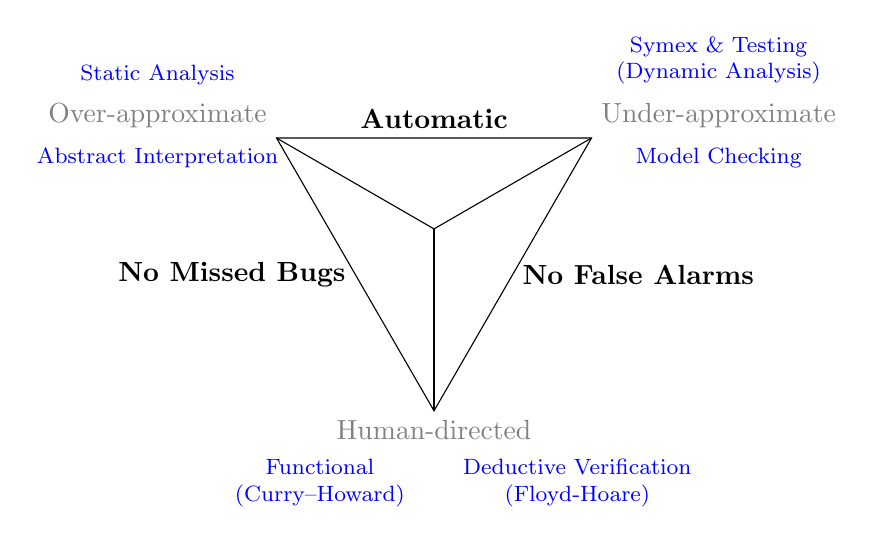
\begin{tikzpicture}
\draw (0,{sqrt(12)}) node[anchor=south east, label=above:{\color{blue} \footnotesize Static Analysis}, label=below:{\color{blue} \footnotesize Abstract Interpretation}] {\color{gray} Over-approximate}
  -- (2,0) node[anchor=north, label={[align=center, text=blue, font=\footnotesize]below left:Functional\\(Curry–Howard)}, label={[align=center, text=blue, font=\footnotesize]below right:Deductive Verification\\(Floyd-Hoare)}] {\color{gray} Human-directed} node[midway, left]{\textbf{No Missed Bugs}}
  -- (4,{sqrt(12)}) node[anchor=south west, label={[align=center, text=blue, font=\footnotesize]above:Symex \& Testing\\(Dynamic Analysis)}, label=below:{\color{blue} \footnotesize Model Checking}] (UA) {\color{gray} Under-approximate} node[midway, right]{\textbf{No False Alarms}}
  -- cycle node[midway, above]{\textbf{Automatic}};

\draw [-] (0, {sqrt(12)}) to (2, 2.31);
\draw [-] (2, 0) to (2, 2.31);
\draw [-] (4, {sqrt(12)}) to (2, 2.31);


% \pgfmathparse{sqrt(12)}
% \node (A) {A};
% \node [right=4cm of A] (B) {B};
% \node [below right=\pgfmathresult cm and 2cm of A] (C) {C};


% \draw [-] (A) to (B) node[midway, right]{this works};
% \draw [-] (B) to (C) node[midway, right]{this works};
% \draw [-] (A) to (C) node[midway, right]{this works};
  
%   \node[fill=blue,circle,text width=3cm] (first) at (1,1) {First};
% \node[fill=green,circle,text width=3cm] (second) at (5,5) {This is the text that will be cover with the connection lines};
% \node[fill=purple,circle,text width=3cm] (third) at (1,9) {This text will be covered too};
% % insert connection lines in background using myback layer

% \draw (first.east) to (third.east);
% \draw (first.west) to (third.north east);

\end{tikzpicture}
\caption{The Triangle Model of Software Verification adapted from the paper by M. Brain and D. Kroening \cite{TSVP}.}
\label{fig:tmsv}
\end{figure}

% \subsection{A Triangle Model of Software Verification}
There are numerous verification techniques, based on formal or informal methods, available into to achieve the ultimate goal of software verification. These techniques can be divided into three categories according to their approach: \textit{Static Analysis}, \textit{Dynamic Analysis}, and \textit{Human-directed Analysis}. Although each of them has their focuses, strengths and weaknesses, their verification achievements can be concluded in three main properties: being automatic, not missing bugs, and excluding false alarms by M. Brain and D. Kroening \cite{TSVP}. These can also be visualised in a triangle model, which has been illustrated in  Figure~\ref{fig:tmsv} below. Since there always is a trade-off between the three proprieties, it becomes a weakness of such techniques. They can be considered as sitting at a corner of the triangle and climbing to the top of a pyramid while they are trying to tackle their weakness. We will discuss each of them with some  highlighted techniques as examples and the use of software verification in the following subsections.

% , while these existing techniques can be defined into six categories: 1) Static Analysis, 2) Abstract Interpretation, 3) Testing \& Symbolic Execution (Symex), 4) Model Checking, 5) Functional and 6) Deductive Verification. 

% is designed for a particular purpose. We discuss those techniques which are highly researched or presented recently.
% % A Survey of Automated Techniques for Formal Software Verification
% A survey that conducted by V. D'Silva et al. \cite{4544862} gave a detailed overview of three main automatic formal verification techniques, and brought out their strengths and weaknesses for applying to practical problems. The three techniques are: 1) Static Analysis, 2) Model Checking, and 3) Bounded Model Checking. 

\input{contents/2.1.softwareVerificationTechniques}

\subsection{The Use of Software Verification}
Software verification are commonly used for two main purposes: 1) hunting bugs, and 2) proving the program functional correctness. Below are several case studies making good use of the model checking, which is the technique we focused on in this project:

\subsubsection{Hunting bugs}
% Towards Improving Software Security using Language Engineering and mbeddr C
M. Voelter et al.\cite{Voelter:2015:TIS:2846696.2846698} took several well-know bugs as examples to show how the modular extension of the C programming language can improve software security. One of the examples is the Heartbleed bug in OpenSSL TLS mentioned in Section~\ref{sec:heartbleed bug}. By constructing a simple harness and a message with a nondeterministic data buffer, CBMC is able to identify the failure in a short period. This is a great demonstration of the importance of formal verification in the software development. 

% SAT-based Bounded Software Model Checking for Embedded Software: A Case Study
Another remarkable case study presented by Y. Kim and M. Kim \cite{7091291} has successfully detected four hidden bugs in an embedded software, lazybox ls, using CBMC. This study highlighted the pivot of loops analysis, determining the minimum iterations to exit a loop, to avoid false negative detections in practice. As an accurate unwinding loop bound can minimise the chances of missing bugs, state explosion, and execution timeout. The experiment also showed the effectiveness of using such model checking technique and its limitation on the loop analysis. 

% Using Model Checking to Find Serious File System Errors
There is a case study conducted by J. Yang et al. \cite{Yang:2006:UMC:1189256.1189259} demonstrated a systematical way to model check three widely-used and heavily-tested file systems. Two classes of checks are suggested: 1) generic checks for those general properties should hold at any point, and 2) consistency checks for the functional properties that the file system specified. Concerning the complexity of such file systems, it is impractical to be fully tested in the traditional way as there could be an exponential number of test cases for checking the recovery mechanism. Model checking make use of several state-reducing techniques, which makes it capable to explore such vast state spaces efficiently. As a result, 32 serious bugs are found during the experiment.

\subsubsection{Proving correctness}
% very useful experiment
% Verifying Code and Its Optimizations: An Experience Report
An experience report presented by R. Metta \cite{Metta:2011:VCO:2004685.2005455} described their experience in verifying the correctness of a 200-line implementation of Cyclic Redundancy Check. The study indicated that sometime the specification and verification process can hardly be automated and required intense human efforts even for such a small code bases. It is hard to scale up if such a program containing huge loops. The authors further suggested a bottom-up approach to verify the correctness of each functions independently through CBMC first, and then to verify the correctness of the loop through an induction manually using CBMC. 

% Verification of Safety-Critical Systems: A Case Study Report on Using Modern Model Checking Tools
A. J{\"a}{\"a}skel{\"a}i et al. \cite{jskelinen_et_al:OASIcs:2012:3589} verified the implementation of the 2003 voting scheme in a systematic capability 3 level shutdown system through model checking. The experiment is conducted in two stages: 1) refine and translate the requirements into pseudo code directly for a preliminary verification, and then move on to 2) verify the actual implementation of the voting scheme. The study concluded in several suggestions for using model checking techniques. Beginning with some simple test cases can help to understand how to give precise and effective assertions before jumping into those complicated properties. Fault seeding techniques is recommended for inexperienced users in order to check the correctness of assertions by introducing violation to the corresponding properties. 
% done

% Automated Verification for Functional and Relational Properties of Voting Rules
Another study conducted by B. Beckert et al. \cite{beckertBormerKirsten2016} verified the functional and relational properties of voting rules, and demonstrated the effectiveness of using bounded model checking and deductive verification. Moreover, it also showed that the verification effort can be greatly reduced by using symmetry properties. 

% can be very accurate, but it requires certain times and memory space for exploring the possible states.
F. Werner and D. Farago \cite{Werner2010CorrectnessOS} investigated CBMC to the domain of wireless sensor networks (WSNs) and proved that it is capable to perform automatic verification on a system about 21000 LoC. It showed that the scalability can be greatly improved by the proposed abstractions and simplification heuristics, with the --slice-formula option enabled. The study further concluded that CBMC with the abstractions and heuristics is powerful enough to verify large scale programs. 

\subsubsection{Other applications}
There are several studies showing that model checking is applied to various usages, such as embedded software verification \cite{Cordeiro:2009:SBM:1747491.1747515, BK11}, cross-platform verification \cite{0fbeb641779543c98fb1d6ff2180664c}, sequentialisation-based verification \cite{6693139}, fault localisation \cite{Griesmayer:2007:AFL:1247747.1248089}, equivalence checking \cite{Lee2011}, cyber-physical system co-verification \cite{6649878}, and test-vector generation \cite{Angeletti2009}.

% Show wt CBMC / Bounded model checking can do

\section{Related Work}
The use of model checking technique for automated formal verification of software has been presented and widely researched over the last couples of decades. In this section, we discuss some practical applications and experiences of applying model checking techniques on security audit and assurance. It is important to learn from the successful cases from others in order to observe how the model checking is being used effectively and what kind of effect it has contributed to the development process and the overall quality.

\subsection{Formal software verification techniques}
There are numerous formal verification techniques available for software verification. Each of them is designed for a particular purpose. We discuss those techniques which are highly researched or presented recently.
% A Survey of Automated Techniques for Formal Software Verification
A survey that conducted by V. D'Silva et al. \cite{4544862} gave a detailed overview of three main automatic formal verification techniques, and brought out their strengths and weaknesses for applying to practical problems. The three techniques are: 1) Static Analysis, 2) Model Checking, and 3) Bounded Model Checking. We discuss each of them in detail below.

% What is it
% How it works
% Limitation?
% Advantages.
% Compare with BMC
% Some statictis

% Comparing Model Checking and Static Program Analysis: A Case Study in Error Detection Approaches
\paragraph{Static analysis} generally refers to a family of techniques for determining the run-time properties of a program without executing it. Static analysis is able to indicate run-time errors automatically at compilation time without any code instrumentation or user interaction. Therefore, these techniques are commonly used in compiler optimisation. In term of software verification, the soundness of an analysis relies on the approximation, which becomes a limitation to static analysis. As the undecidability of static analysis problems, it is not possible to come up with an approximation that produces no false positive and no false negative detections. It uses some simple predefined fact for showing the absence of simple errors, such as no assertion violation, no arithmetic overflow, and no exceed of array bounds, efficiently. However, it is difficult to generate counterexamples, due to the precision loss during the analysis which is a significant trade-off for efficiency.

In contrast to static analysis, model checking is more precise as it can prove more complicated properties and provides counterexamples once a bug is found. The above statements are supported by the experimental result conducted by K. Vorobyov and P. Krishnan \cite{vorobyov2010comparing}. The experiment compares the verification result of static program analysis with the one of model checking by applying Parfait and CBMC respectively on some benchmarked code base. By configuring CBMC to focus on particular types of error, it showed a high accuracy rate (97\% overall true positive detections, and found about 19\% more bugs), whereas only 77\% with Parfait. Moreover, both of them reported a 0\% false positive detections, which is common for model checking and a specific design to minimise it for static program analysis. However, model checking is much more expensive with respect to computation time and memory usage, as it reached the memory limit in the experiment. The study further concluded that: 1) scalability can be a problem for model checking a large size code base, such as an operating system, and 2) an insufficient unwinding was one of the reasons for false negative detections of CBMC.

\paragraph{Model Checking} is a technique for verifying the correctness of a finite-state system as mentioned in Section~\ref{sec:mc}. It computes the run-time states of the software without actually running the program. Each reachable state is examined whether a correctness property holds. If such an execution path violating any of the properties is found, a counterexample is formed. This process is guaranteed to terminate only if there are finite states. This technique is frequently used on verifying the safety properties of device drivers and systems code. However, it is easy to run into a state space explosion problem while analysing a medium sized code bases \cite{Yeolekar2013}. Even with the help of SAT or SMT solver and some abstraction techniques, model checking is hard to scale up to the size level that static analysis does. 

\paragraph{Bounded Model Checking} is a complementary technique to model checking with an upper bound of the number for explored state as mentioned in Section~\ref{sec:bmc}. It unrolls the transition operations for $k$ times and combines the properties to form a propositional formula, which is solvable by a SAT solver. The formula is satisfiable as long as the property is violated by a trace of length $k$. Such technique is sound for the execution paths up to the specified length $k$, while a bug can exist beyond the bound. Although it may result in an inconclusive outcome, BMC is still a great successful technique for finding bugs, as well as proving the liveness and safety properties by applying in different manner. V. D'Silva et al. \cite{4544862} further concluded that bounded model checking is the best technique to find shallow bugs comping with static analysis and model checking, and is able to provide a complete counterexample trace once a bug is found. However, the completeness is not guaranteed if the program contains deep loops.

% very useful paper, about abstraction
% The concept of dynamic analysis
\paragraph{Dynamic analysis} is a technique to analyse the run-time proprieties by executing a program, which is in contrast to static analysis. It is not able to prove a particular property holds, but nevertheless it is useful for detecting violations of properties \cite{Ball:1999:CDA:318774.318944} and able to scale to large-size code bases. A. Yeolekar and D. Unadkat \cite{Yeolekar2013} presented a counterexample-guided abstraction refinement (CEGAR) based technique by utilising dynamic analysis to overcome the scalability limitation of model checking. Dynamic inference is used to guess invariants and refine the abstraction from spurious counterexamples, thus a better precision of the abstraction and an accelerated loop refinement are achieved in their experiment.

% Concolic Testing of the Multi-sector Read Operation for Flash Memory File System
% comparing concolic testing with model checking
\paragraph{Concolic testing} is a hybrid software verification technique joining symbolic static analysis and concrete dynamic analysis, which is able to generate test cases automatically and to examine execution paths exhaustively. M. Kim et al. \cite{Kim:2009:CTM:1693660.1693677} conducted an experiment on concolic testing to analyse the multi-sector read operation for a flash memory, and summarised its advantages and weaknesses compared to model checking techniques. Concolic testing algorithm in general consists of five steps: 1) Instrumentation, 2) Concrete execution, 3) Symbolic execution, 4) Deciding the next execution path, and 5) Choosing the next input values. As the symbolic execution preforms along the concrete execution path, no false alarms will be produced. Once the path formulas are not able to be solved by a constraint solver, some symbolic constraints will be simplified by replacing some of the symbolic values with concrete value. This may leads to an incomplete coverage. The experimental result showed it had a better applicability and lower memory usage. However, the study also reflected that concolic testing is a time-consuming method as time will be wasted on generating invalid test cases in a complex environment model. %Concolic testing can analyse a software with underlying binary libraries without any manual abstraction, which is necessary for model checking. 
Concolic testing can be a good choice for finding bugs, but not for demonstrating program correctness. Model checking generally provides high accuracy and a better performance of the verification than concolic testing, which is essential for verifying critical software.

\subsection{Software Verification approaches through MC}

% Traditional testing vs Abstract testing.
% Bridging the gap between test cases and requirements by abstract testing
\paragraph{Abstract testing} is a software testing approach proposed by F. Merz et al. \cite{Merz:2015:BGT:2837773.2837824}, which focuses on the relation between requirements and the corresponding test cases in order to replace the traditional test cases by an abstract one. Each abstract test cases is derived form the requirements and formulated into assumption and assertion statements on the source code level, which is often a one to one relation. Assumption and assertion statements are the constraints encoding the preconditions and postconditions respectively. Setting up these constraints for the testing environment with respect to non-deterministic values, rather using concrete values. Hence, an abstract test case is possible to represent a large number of concrete test cases, which can remarkably simplify the test cases generation and maintenance process. The experimental study showed that abstract testing is more capable and efficient to discover underlying bugs than traditional software testing. Moreover, the performance of CBMC is promising with less than 20s runtime on average for an abstract test case, which is suitable for agile-like development process. Once there is a change of requirement, it is easily and directly visible to the corresponding abstract test cases.

%  ********** may be related
% Unit Testing of Flash Memory Device Driver through a SAT-Based Model Checker
Besides the incomplete coverage of conventional testing stated above, M. Kim et al. \cite{4639323, Kim:2008:FVF:1429078.1429092, 5510242} also mentioned that once a violation is detected, it still require a large amount of human effort to locate where the violation occurred by replaying the scenario and tracing the execution step-by-step. Hence, model checking techniques is well-suited to overcoming these weaknesses of conventional testing method through exhaustive analyses. This study applied SAT-based bounded model checking technique to verify the functional correctness and increase the reliability of the device driver software for Samsung's OneNAND\textsuperscript{TM} flash memory. In order to extract the code level properties, the study also suggested a top-down approach to identify the properties from several design documents, such as software requirement specifications, architecture design specifications, and detailed design specifications. It demonstrated a practical way on how the functional correctness properties can be extracted from the real world environment. By replacing the conventional testing with constraint-based exhaustive testing, which is the same as abstract testing above, CBMC achieved a great success in the experiment that discovered some bugs including incomplete exceptions handling and logical bugs. This promising result shows that model checking techniques are mature enough to be applied on verifying an industrial level software.

% Unit Testing of Flash Memory Device Driver through a SAT-Based Model Checker
% One advantage of SAT-based model checking is that a target C code can be analysed directly without an abstract model, thereby enabling automated and bit-level accurate verification. 
% Software requirement specifications (SRS), Architecture design specifications (ADS), Detailed design specifications (DDS)

% Property-based Code Slicing for Efficient Verification of OSEK/VDX Operating Systems
% very useful paper and also about CBMC
\paragraph{Property-based code slicing}
Despite the fact that model checking is a powerful technique, it often requires more knowledge and cost than testing. In order to reduce the cost while maintain comprehensiveness, M. Park et al. \cite{DBLP:journals/corr/abs-1301-0042} proposed an approach that consists of three strategies: 1) property-based environment generation, 2) property-based abstraction, and 3) collaborative verification using model checking and testing. The study applied it to verify the Trampoline operating system. The result showed that the approach is able to reduce the verification cost by scaling down the target code, and to simplify the analysis process by localising the verification activity.

% working on it.

% property-based environment generation and model extraction techniques using static code analysis, which can be applied to both model checking and testing. Comparative experiments using random testing and model checking for the verification of assertions in the Trampoline kernel code show how our environment generation and abstraction approach can be utilised for efficient fault detection. 

% Testing is insufficient for identifying subtle issues due to its optimistic incompleteness.

% Model checking is a powerful technique that supports comprehensiveness, and is thus suitable for the verification of safety-critical systems. However, it generally requires more knowledge and cost more than testing.

\paragraph{False positive elimination}
Software verification based on abstract interpretation is scalable for verifying industrial level code bases, but imprecise. Many spurious errors are generated as the abstract interpretation over-approximated the execution traces than the program can actually perform. Manual investigation is needed to review each error, such manual efforts are costly to the development process. To overcome this problem, 
% Reducing false positive
% Reducing False Positives by Combining Abstract Interpretation and Bounded Model Checking
H. Post et al. \cite{4639322} and P. Darke et al. \cite{Kumar:2013:PRA:2491411.2494569} integrate model checking to reduce the number of false positive generated by the static analysis tools. The experimental result shows that 69\% of warnings have been successfully removed by CBMC. 

% Reducing False Positives by Combining Abstract Interpretation and Bounded Model Checking
% The study shows that CBMC can generally provide more counter-example than SATABS. Abstract interpretation uses an over-approximation on the set of possible execution trace. i.e., it considers more program execution paths than the program can actually perform. Introduce false positives.

% doi not found, false positive elimination
% Efficient Elimination of False Positives Using Bounded Model Checking
Another study by T. Muske et al \cite{tukaram2013efficient} points out the above approach could involve numerous verifications, and further proposes an approach consisting of three techniques to achieve a faster false positives elimination. By avoiding redundant equivalent assertions, results in a 60\% accelerated false positives elimination. 

% identify an assertion as being equivalent to an other assertion thus avoiding its verification. Then, tries to identify and skip a class of assertion verifications that will not eliminate a false positive.

% Software verification using abstract interpretation is scalable but imprecise. Model checking is precise in verifying a property but not scalable. Often, these two techniques are combined to achieve better precision.

% On the Formal Verification of Component-based Embedded Operating Systems
% system level verification - isolation of components for modular verification
\paragraph{Aspect-oriented programming technique} M. Ludwich and A. Frohlich \cite{Ludwich:2013:FVC:2433140.2433148} introduced an approach to formally verify both \textit{functional correctness} and \textit{safety properties} of embedded operating system components. Such components are supposed to be shifted between different domains, therefore, the implementation of formal verification must also be domain-independent. The study proposed a corresponding strategy that consists of three main steps: 1) creating contracts for each components that to be verified , 2) implementing such components with the corresponding contracts accordingly, and 3) performing software bounded model checking to verify whether the implementation of components respect to their contracts. The benefits of keeping the specification and implementation close to each other is that any violations in the implementation can be detected at the early stage of development. However, this may introduce an extra run-time overhead to its instances. Hence, those contracts should be partially eliminated from the implementations beyond the verification stage. The experiment made used of aspect-oriented programming technique to achieve this purpose, and further facilitate a modular verification by isolation different components. Note that components isolation is not suitable for verifying a monolithic design. More importantly, the experiment also demonstrated that the functional correctness and safety properties can be verified by the contracts captured from requirements and those properties generated by the model checker respectively. This approach is a kind of white box testing and is more suitable to carry out at the early stage or during the development.

% How Verified is My Code? Falsification-Driven Verification (T)
\paragraph{Falsification-Driven Verification} A. Groce et al. \cite{7372062} stated the idea of a "verification successful" in model checking or even theorem proving can be a sign of insufficient verification properties. In order to gain more knowledge of the meaning behind "successful" results, the study proposed a falsification-driven methodology that adapts mutation testing to show the weakness of current specification. Mutate both the harness and the program with a small syntactic change assuming a good test suit should be able to detect a bug introduced by such a change. Hence, the mutation kill rate can act as a measurement unit of the accuracy rate and correctness of a harness. As a better harness should able to detect more errors from the implementation. This approach is useful for ensuring the quality of harnesses, thus a more reliable verification. However, it requires many manual efforts to verify and examine the mutants while some of them can be semantically equivalent. It would be suitable for developers who are not familiar with formal verification but intend to verify a system.

% On the Formal Verification of Component-based Embedded Operating Systems
% Moreover, they demonstrate the approach causes no run-time overhead, since the adopted Software Model Checking techniques are deployed at compile-time. The functional correctness properties of a component are expressed by a contract containing assertions that represent class invariants, pre, and postconditions for each method declared in the component's interface. The safety properties are meant to be automatically generated by model checker.


% A contract is composed by the invariants of the class that defines the component and by a set of pre and postconditions. Class invariants are defined as a set of assertions that are always true for all instances of that class. The preconditions of a method define a set of assertions that must be true in case the method invocation terminated normally (ie. without triggering exceptions, which have not yet been addressed in our approach.) Pre and postcondition assertions can reason about the method's parameters, return value, and object state.

% Bridging the gap between test cases and requirements by abstract testing
% The havoc() procedure call in the example sets some global vari- ables to undefined (non-deterministic) values.

% \begin{itemize}
%     \item Software testing only consists of few selected cased for checking the correctness, which is sound but not complete.
%     \item Abstraction based verification techniques covers all possible input spaces, which is complete but may cause false positive.
%     \item Bounded Model Checking is sound, but only execution paths up to the specified length are checked; therefor not complete.
%     \item BMC with large enough bound is sound and complete.
% \end{itemize}


% no really helpful - configuration lifting
% Configuration Lifting: Verification meets Software Configuration
\paragraph{Configuration lifting} is a specification analysis technique presented by
H. Post and C. Sinz \cite{4639338}, which transforms all variants into a meta-program and facilitates the following specification analysis in three different domains: 1) inconsistencies within a feature model, 2) inconsistencies between the feature model and their implementations, and also 3) the coverage of run-time errors in all product variants. The study demonstrated the technique on verifying Linux kernel and device driver, which successfully found two bugs in the kernel configuration system. The experimental result showed that this technique is able to apply on a large size system included more than 4600 features and model checking on the meta-program provides a significant speed-up compared with traditional enumeration based analysis.

% Semiformal Verification of Embedded Software in Medical Devices Considering - Stringent Hardware Constraints
\paragraph{Other approaches} L. Cordeiro et al. \cite{5066674} propose a semi-formal verification approach combined dynamic and static verification to stress and cover the state spaces of embedded software exhaustively, in order to improve the coverage and reduces the verification time. This approach allows developers to reason both the functional and temporal properties quantitatively to guarantee the timeliness and correctness of the design. The experimental result shows that model checkers have  limitation to specify more complex temporal properties and state space explosion problem.

\subsection{Practical software verification}
Software verification can generally be categorised into two main purposes: 1) hunting bugs, and 2) proving the program correctness. Below are several case studies which are making good use of the model checking are discussed below:

\subsubsection{Hunting bugs}
% Towards Improving Software Security using Language Engineering and mbeddr C
M. Voelter et al.\cite{Voelter:2015:TIS:2846696.2846698} took several well-know bugs as examples to show how the modular extension of the C programming language can improve software security. One of the examples is the Heartbleed bug in OpenSSL TLS mentioned in Section~\ref{sec:heartbleed bug}. By constructing a simple harness and a message with a nondeterministic data buffer, CBMC is able to identify the failure in a short period. This is a great demonstration of the importance of formal verification in the software development. 

% SAT-based Bounded Software Model Checking for Embedded Software: A Case Study
Another remarkable case study presented by Y. Kim and M. Kim \cite{7091291} has successfully detected four hidden bugs in an embedded software, lazybox ls, using CBMC. This study highlighted the pivot of loops analysis, determining the minimum iterations to exit a loop, to avoid false negative detections in practice. As an accurate unwinding loop bound can minimise the chances of missing bugs, state explosion, and execution timeout. The experiment also showed the effectiveness of using such model checking technique and its limitation on the loop analysis. 

% Using Model Checking to Find Serious File System Errors
There is a case study conducted by J. Yang et al. \cite{Yang:2006:UMC:1189256.1189259} demonstrated a systematical way to model check three widely-used and heavily-tested file systems. Two classes of checks are suggested: 1) generic checks for those general properties should hold at any point, and 2) consistency checks for the functional properties that the file system specified. Concerning the complexity of such file systems, it is impractical to be fully tested in the traditional way as there could be an exponential number of test cases for checking the recovery mechanism. Model checking make use of several state-reducing techniques, which makes it capable to explore such vast state spaces efficiently. As a result, 32 serious bugs are found during the experiment.

\subsubsection{Proving correctness}
% very useful experiment
% Verifying Code and Its Optimizations: An Experience Report
An experience report presented by R. Metta \cite{Metta:2011:VCO:2004685.2005455} described their experience in verifying the correctness of a 200-line implementation of Cyclic Redundancy Check. The study indicated that sometime the specification and verification process can hardly be automated and required intense human efforts even for such a small code bases. It is hard to scale up if such a program containing huge loops. The authors further suggested a bottom-up approach to verify the correctness of each functions independently through CBMC first, and then to verify the correctness of the loop through an induction manually using CBMC. 

% Verification of Safety-Critical Systems: A Case Study Report on Using Modern Model Checking Tools
A. J{\"a}{\"a}skel{\"a}i et al. \cite{jskelinen_et_al:OASIcs:2012:3589} verified the implementation of the 2003 voting scheme in a systematic capability 3 level shutdown system through model checking. The experiment is conducted in two stages: 1) refine and translate the requirements into pseudo code directly for a preliminary verification, and then move on to 2) verify the actual implementation of the voting scheme. The study concluded in several suggestions for using model checking techniques. Beginning with some simple test cases can help to understand how to give precise and effective assertions before jumping into those complicated properties. Fault seeding techniques is recommended for inexperienced users in order to check the correctness of assertions by introducing violation to the corresponding properties. 
% done

% Automated Verification for Functional and Relational Properties of Voting Rules
Another study conducted by B. Beckert et al. \cite{beckertBormerKirsten2016} verified the functional and relational properties of voting rules, and demonstrated the effectiveness of using bounded model checking and deductive verification. Moreover, it also showed that the verification effort can be greatly reduced by using symmetry properties. 

% can be very accurate, but it requires certain times and memory space for exploring the possible states.
F. Werner and D. Farago \cite{Werner2010CorrectnessOS} investigated CBMC to the domain of wireless sensor networks (WSNs) and proved that it is capable to perform automatic verification on a system about 21000 LoC. It showed that the scalability can be greatly improved by the proposed abstractions and simplification heuristics, with the --slice-formula option enabled. The study further concluded that CBMC with the abstractions and heuristics is powerful enough to verify large scale programs. 

\subsection{Model Checking tools}
\paragraph{CRUST} is a bounded verifier developed by J. Toman et al. \cite{7371997} combines exhaustive test generation and bounded model checking technique in order to detect memory safety errors. It will first generates a set of testing driver for those relevant APIs, converts the driver code from Rust to C, and then performs bounded model checking. With the help of exhaustive test generation, it is able to efficiently explore large input spaces and generated multiple test drivers for covering the input spaces as many as possible. CBMC is used as a back-end service for automated analysis. By evaluating data structures from Rust standard library, CRUST is capable to detect some memory safety bugs from it.

% % A Comparative Study of Software Model Checkers as Unit Testing Tools: An Industrial Case Study
% M. Kim et al. \cite{5510242} reported their experience in applying Blast and CBMC to testing the components of a storage platform software for flash memory.

% Significant additional efforts are required to create an abstract target model, which is not affordable for most industrial projects.



\subsection{Other applications}
There are several studies showing that model checking is applied to various usages, such as embedded software verification \cite{Cordeiro:2009:SBM:1747491.1747515, BK11}, cross-platform verification \cite{0fbeb641779543c98fb1d6ff2180664c}, sequentialisation-based verification \cite{6693139}, fault localisation \cite{Griesmayer:2007:AFL:1247747.1248089}, equivalence checking \cite{Lee2011}, cyber-physical system co-verification \cite{6649878}, and test-vector generation \cite{Angeletti2009}.


% \cite{5510242}
% There have been several studies in which an SMC was
% applied to various target systems such as automotive
% software [47], microcontroller programs [48], Linux device
% drivers [45], [46], file systems [52], network filters [13], a
% protocol stack [40], and server applications [41]. For a flash
% storage platform, which is our main target domain, one
% recent study [32] analyzes flash file systems as an effort of
% the mini-challenge [35]. However, the majority of verification
% research [36], [28], [11] on flash file systems focus on
% the specifications of the file system design and not on an
% actual instance of implementation.

% % not really helpful
% *T. Vortler et al. \cite{7195716} presented a verification framework for applications for the embedded system operating system Contiki, based on CBC, supporting interrupts.

% % not really helpful (something about partial reduction) - verifying sensor node using CBMC
% % D. Bucur and M. Kwiatkowska \cite{BK11}

% % not really helpful - but a bit about CBMC
% *B. Schlich and S. Kowalewski \cite{Schlich:2009:MCC:1569778.1569782} studied 14 tools and summarised the limitations for verifying embedded software.


% % Crowdsourcing Program Preconditions via a Classification Game
% % D. Fava et al. \cite{Fava:2016:CPP:2884781.2884865} used CBMC to generate the Invariant / check whether the precondition can cause the postcondition

% % % Seems not really helpful
% % I. Wenzel et al. \cite{0fbeb641779543c98fb1d6ff2180664c} 
% % only use CBMC for test data generation.

% % talked about memory safety
% *H. Post and W. K \cite{Post:2007:ISA:1770498.1770525} able to verify the memory safety of Linux drivers using CBMC.

% % Something about CBMC maybe useful
% *L. Cordeiro et al. \cite{Cordeiro:2009:SBM:1747491.1747515}
% CBMC has limitations due to the fact that the size of the propositional formulae increases significantly in the presence of large datapaths and high-level information is lost when the verification conditions are converted into propositional logic.


% \cite{Petrenko:2015:MTA:2744769.2747935}


% % Not very helpful, may be talk about some scale up problem & comparison with CBMC
% *P. Cousot et al. \cite{ousotEtAl10-FMSDC}


% % To the best of our knowledge, there is no work that considers .... As a result, our main contribution is ....